\documentclass{experimentreport}

\usepackage{listings}
\usepackage{xcolor}

\definecolor{codegreen}{rgb}{0,0.6,0}
\definecolor{codegray}{rgb}{0.5,0.5,0.5}
\definecolor{codepurple}{rgb}{0.58,0,0.82}
\definecolor{backcolour}{rgb}{0.95,0.95,0.92}
\definecolor{lightgreen}{rgb}{0,0.4,0}
\definecolor{lightred}{rgb}{0.4,0,0}

\definecolor{mygray}{gray}{.9}

% \lstdefinestyle{mystyle}{
\lstset{
    %backgroundcolor=\color{backcolour},   
    commentstyle=\color{brown},
    keywordstyle=\color{magenta},
    numberstyle=\tiny\color{codegray},
    stringstyle=\color{codepurple},
    basicstyle=\ttfamily\tiny,
    breakatwhitespace=false,         
    breaklines=true,                 
    captionpos=b,                    
    keepspaces=true,                 
    numbers=none,                    
    numbersep=5pt,                  
    showspaces=false,                
    showstringspaces=false,
    showtabs=false,                  
    tabsize=2,
    escapeinside={<@}{@>}
}

% \lstset{
% basicstyle=\ttfamily\bfseries\footnotesize,
%   morekeywords={virtualinvoke},
%   keywordstyle=,
%   ndkeywordstyle=\color{red},
%   commentstyle=\color{gray},
%   stringstyle=\color{green},
%   numbers=none,
%   breaklines=true,
%   numberstyle=\ttfamily\footnotesize\color{gray},
%   stepnumber=1,
%   numbersep=6pt,
%   backgroundcolor=\color{white},
%   tabsize=4,
%   showspaces=false,
%   showstringspaces=false,
%   xleftmargin=6pt,
%   captionpos=t
% }

\lstdefinelanguage{JavaScript}{
  keywords={typeof, new, true, false, catch, function, return, null, catch, switch, var, if, in, while, do, else, case, break, export, static, const, let, class, void, async, await, interface, extends, public, this},
  % basicstyle=\linespread{1.0}\ttfamily\footnotesize,
  % keywordstyle= \color{violet}\bfseries,
  ndkeywords={class, export, boolean, throw, implements, import, this},
  ndkeywordstyle=\color{darkgray}\bfseries,
  identifierstyle=\color{black},
  sensitive=false,
  frame=lines,
  comment=[l]{//},
  morecomment=[s]{/*}{*/},
  % commentstyle=\color{gray}\ttfamily,
  % stringstyle=\color{blue}\ttfamily,
  morestring=[b]',
  morestring=[b]"
}



\usepackage{graphicx}
\usepackage{hyperref}
\usepackage{enumitem}

%========================
% 基本信息
%========================

\setcoursename{基础软件开发技术实践}
\setreportname{智能软件工程实验报告}

\setexperimenttitle{实验一：代码审查意见挖掘与需求理解}

\setstudentname{\hintholder{廖正强}}
\setdepartment{\hintholder{计算学部}}
\setstudentid{\hintholder{2023112920}}

\setcourseteacher{刘佳琨}
\setinstructor{刘佳琨}

\setlablocation{\hintholder{格物213}}
\setlabtime{    \hintholder{2026/7/3}}

\begin{document}

%========================
% 自动生成封面
%========================

\makereporthead

%========================
% 实验目的
%========================

\experimentpurpose{

本实验是“代码审查（Code Review）”研究系列的第一个实验，旨在构建一个包含丰富信息的代码审查数据集，该数据集将作为后续所有实验的唯一数据来源。

具体目标包括：
\begin{enumerate}[label=(\arabic*)]
    \item 熟悉 GitHub Pull Request 的组织形式，理解 PR、Review、Commit 之间的关系；
    \item 通过 GitHub API 获取 5 个大型开源项目的 Pull Request 数据；
    \item 获取每条 PR 对应的 Code Review 信息（Review 决策、Reviewer、Inline Comments）；
    \item 获取代码修改内容（修改文件、修改函数、Diff、Commit 信息）；
    \item 提取结构化特征（PR 长度、文件数、Reviewer 数、Comment 数等）；
    \item 对数据集进行统计分析和可视化，为后续的 Merge Prediction 和 Review Comment Generation 任务奠定数据基础。
\end{enumerate}

}

%========================
% 实验内容
%========================

\experimentcontent{

\subsection*{2.1 数据采集}

\textbf{目标项目选择：}选取 5 个具有代表性的大型开源项目：Kubernetes、HuggingFace Transformers、VSCode、Pandas、React。这些项目覆盖了容器编排、自然语言处理、代码编辑器、数据分析、前端框架等不同领域，PR 数量充足，审查流程规范。

\textbf{数据获取流程：}使用 Python 编写数据采集脚本，通过 GitHub REST API v3 进行数据拉取。每条 PR 采集 5 个端点的数据：

\begin{enumerate}[label=步骤\arabic*:]
    \item \textbf{获取 PR 基本信息}（\texttt{GET /repos/\{owner\}/\{repo\}/pulls/\{number\}}）：PR ID、标题、正文、作者、创建时间、合并状态、标签列表。
    \item \textbf{获取 Code Review}（\texttt{GET .../pulls/\{number\}/reviews}）：Reviewer、审查决策（APPROVED / CHANGES\_REQUESTED / COMMENTED）、审查时间、审查评论正文。
    \item \textbf{获取 Inline Review Comments}（\texttt{GET .../pulls/\{number\}/comments}）：代码行级评论，包含文件路径、行号和评论内容。
    \item \textbf{获取代码修改}（\texttt{GET .../pulls/\{number\}/files}）：修改文件列表、增删行数、Unified Diff Patch。
    \item \textbf{获取 Commit 信息}（\texttt{GET .../pulls/\{number\}/commits}）：Commit Message 列表。
\end{enumerate}

\textbf{采集策略：}只采集已关闭（closed）的 PR，随机抽取，每个仓库获取 300 条（总计 1500 条）。采用 3 线程并行采集，每条 PR 内部 5 个 API 调用也并行执行，采集耗时约 15 分钟。配备断点续传机制，支持中断后自动恢复。API 调用共计约 7500 次，使用 GitHub Personal Access Token 认证（5000 次/小时限制），配合限速控制器确保稳定运行。

\subsection*{2.2 特征提取}

对每条 PR 提取以下特征：

\begin{table}[ht]
\centering
\caption{特征字段说明}
\begin{tabular}{|l|l|l|}
\hline
\textbf{类别} & \textbf{特征} & \textbf{来源} \\
\hline
PR 基本信息 & pr\_id, pr\_number, repo, title, body & PR 详情 API \\
\hline
PR 统计量 & pr\_length（标题+正文字符数） & 计算得出 \\
\hline
合并信息 & is\_merged, merge\_status & PR 详情 API \\
\hline
代码修改 & num\_changed\_files, total\_additions, & Files API \\
& total\_deletions, modified\_functions, & Diff 解析 \\
& num\_commits, commit\_messages & Commits API \\
\hline
审查信息 & num\_reviewers, num\_review\_comments, & Reviews API \\
& num\_inline\_comments, review\_decision & Comments API \\
\hline
元标签 & num\_labels, label\_names, & Labels 字段 \\
& has\_ai\_reviewer, has\_ai\_generated\_code & 关键词匹配 \\
\hline
\end{tabular}
\end{table}

\textbf{AI 检测方法：}通过关键词匹配判断 PR 是否涉及 AI。检查 Review 正文、Inline Comment 正文和 PR 标签中是否包含 AI 相关关键词（如 copilot、chatgpt、claude、gpt、llm、codex 等）。AI 生成代码的检测同理，匹配 PR 正文和标签中的 AI 生成关键词（如 ai-generated、generated by ai、gpt- 等）。

\textbf{修改函数提取：}解析 Unified Diff 格式的 Patch，从 Hunk Header（\texttt{@@ -a,b +c,d @@ context}）中提取上下文函数名，同时匹配新增行中的函数定义模式（支持 Python、JavaScript、Go、C/C++、Rust 等语言）。

}

%========================
% 实验结果
%========================

\experimentresult{

\subsection*{3.1 数据集概况}

成功构建包含 \textbf{1500 条 PR} 的结构化数据集（CSV + JSON），涵盖 5 个大型开源项目，每个项目 300 条。数据集包含 26 个字段，覆盖 PR 基本信息、代码审查、代码修改和元标签四大类别。

\subsection*{3.2 总体统计分析}

\begin{table}[ht]
\centering
\caption{数据集总体统计}
\begin{tabular}{|l|c|c|}
\hline
\textbf{指标} & \textbf{数值} & \textbf{占比} \\
\hline
总 PR 数 & 1500 & 100\% \\
\hline
已合并（Merged） & 972 & 64.80\% \\
\hline
未合并 & 528 & 35.20\% \\
\hline
含 AI Reviewer & 523 & 34.87\% \\
\hline
含 AI 生成代码 & 97 & 6.47\% \\
\hline
\end{tabular}
\end{table}
\clearpage
\subsection*{3.3 各仓库对比分析}

\begin{table}[ht]
\centering
\caption{各仓库统计指标对比}
\begin{tabular}{|l|c|c|c|c|c|}
\hline
\textbf{仓库} & \textbf{PR数} & \textbf{合并率} & \textbf{均评论} & \textbf{均审阅人} & \textbf{均长度} \\
\hline
facebook/react & 300 & 48.7\% & 1.04 & 0.71 & 2586.5 \\
\hline
kubernetes/kubernetes & 300 & 66.0\% & 5.11 & 1.41 & 2307.3 \\
\hline
microsoft/vscode & 300 & 87.3\% & 2.79 & 2.29 & 1215.5 \\
\hline
hf/transformers & 300 & 55.3\% & 1.67 & 0.81 & 1806.8 \\
\hline
pandas-dev/pandas & 300 & 66.7\% & 1.53 & 0.85 & 996.0 \\
\hline
\end{tabular}
\end{table}

\subsection*{3.4 数值特征分布}

各数值特征的描述性统计如下：

\begin{itemize}
    \item \textbf{PR 长度}：mean=1782, median=912, range=[9, 44980]。分布呈右偏态。
    \item \textbf{修改文件数}：mean=21.7, median=2.0, range=[0, 3000]。
    \item \textbf{Reviewer 数}：mean=1.21, median=1.0, range=[0, 10]。
    \item \textbf{Review Comment 数}：mean=2.43, median=1.0, range=[0, 133]。
    \item \textbf{标签数}：mean=3.08, median=1.0, range=[0, 43]。
\end{itemize}

\subsection*{3.5 合并 vs 未合并对比}

合并的 PR 与未合并的 PR 在特征上呈现明显差异：
\begin{itemize}
    \item 合并 PR 平均长度（1390）明显短于未合并 PR（2505），说明简洁的 PR 更易被接受。
    \item 合并 PR 平均修改文件数（7.2）远少于未合并 PR（48.2），小步提交更容易通过审查。
    \item 合并 PR 平均 Reviewer 数（1.67）远高于未合并 PR（0.37），有 Reviewer 参与的 PR 更可能被合并。
\end{itemize}

\subsection*{3.6 可视化分析}

\begin{figure}[ht]
\centering

\includegraphics[width=\textwidth]{../figures/01_merge_status_bar.png}
\caption{各仓库合并状态对比柱状图}
\end{figure}

\begin{figure}[ht]
\centering

\includegraphics[width=\textwidth]{../figures/02_comment_distribution_hist.png}
\caption{Review Comment 数量分布直方图}
\end{figure}

\begin{figure}[ht]
\centering

\includegraphics[width=\textwidth]{../figures/03_label_distribution_pie.png}
\caption{Top-10 PR 标签分布饼图}
\end{figure}

\begin{figure}[ht]
\centering
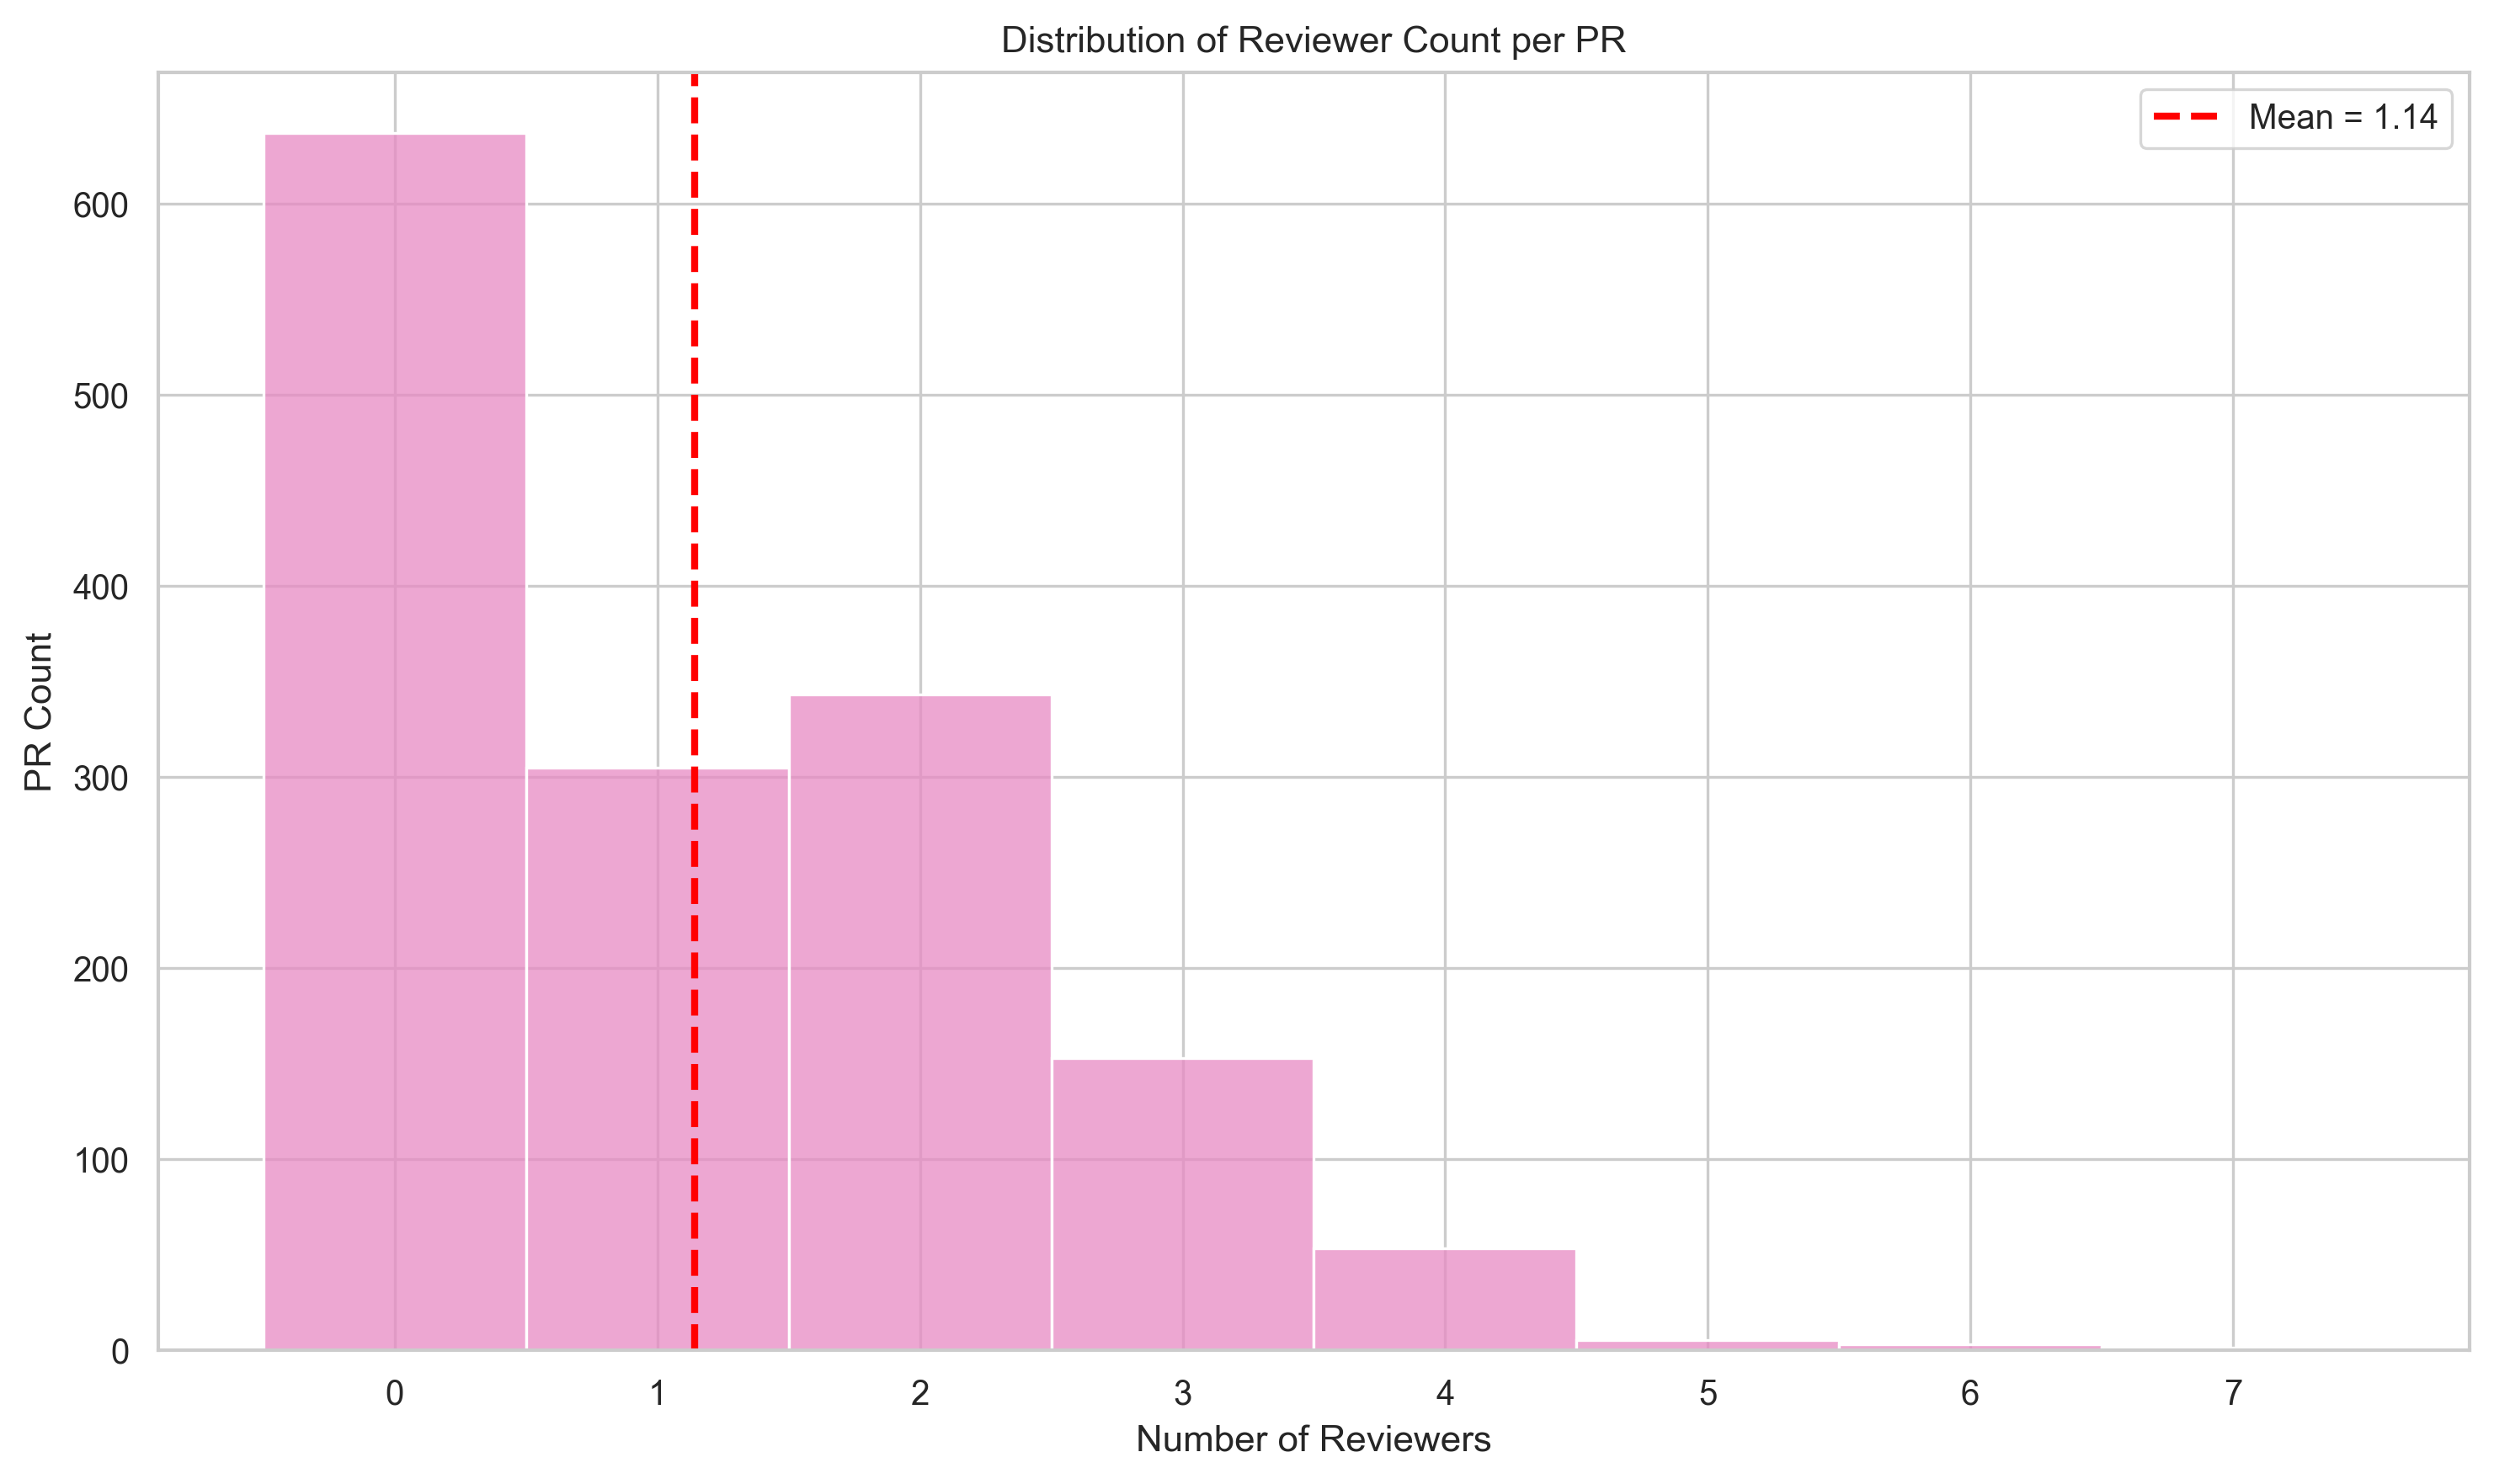
\includegraphics[width=\textwidth]{../figures/04_reviewer_count_distribution.png}
\caption{Reviewer 数量分布}
\end{figure}

\begin{figure}[ht]
\centering
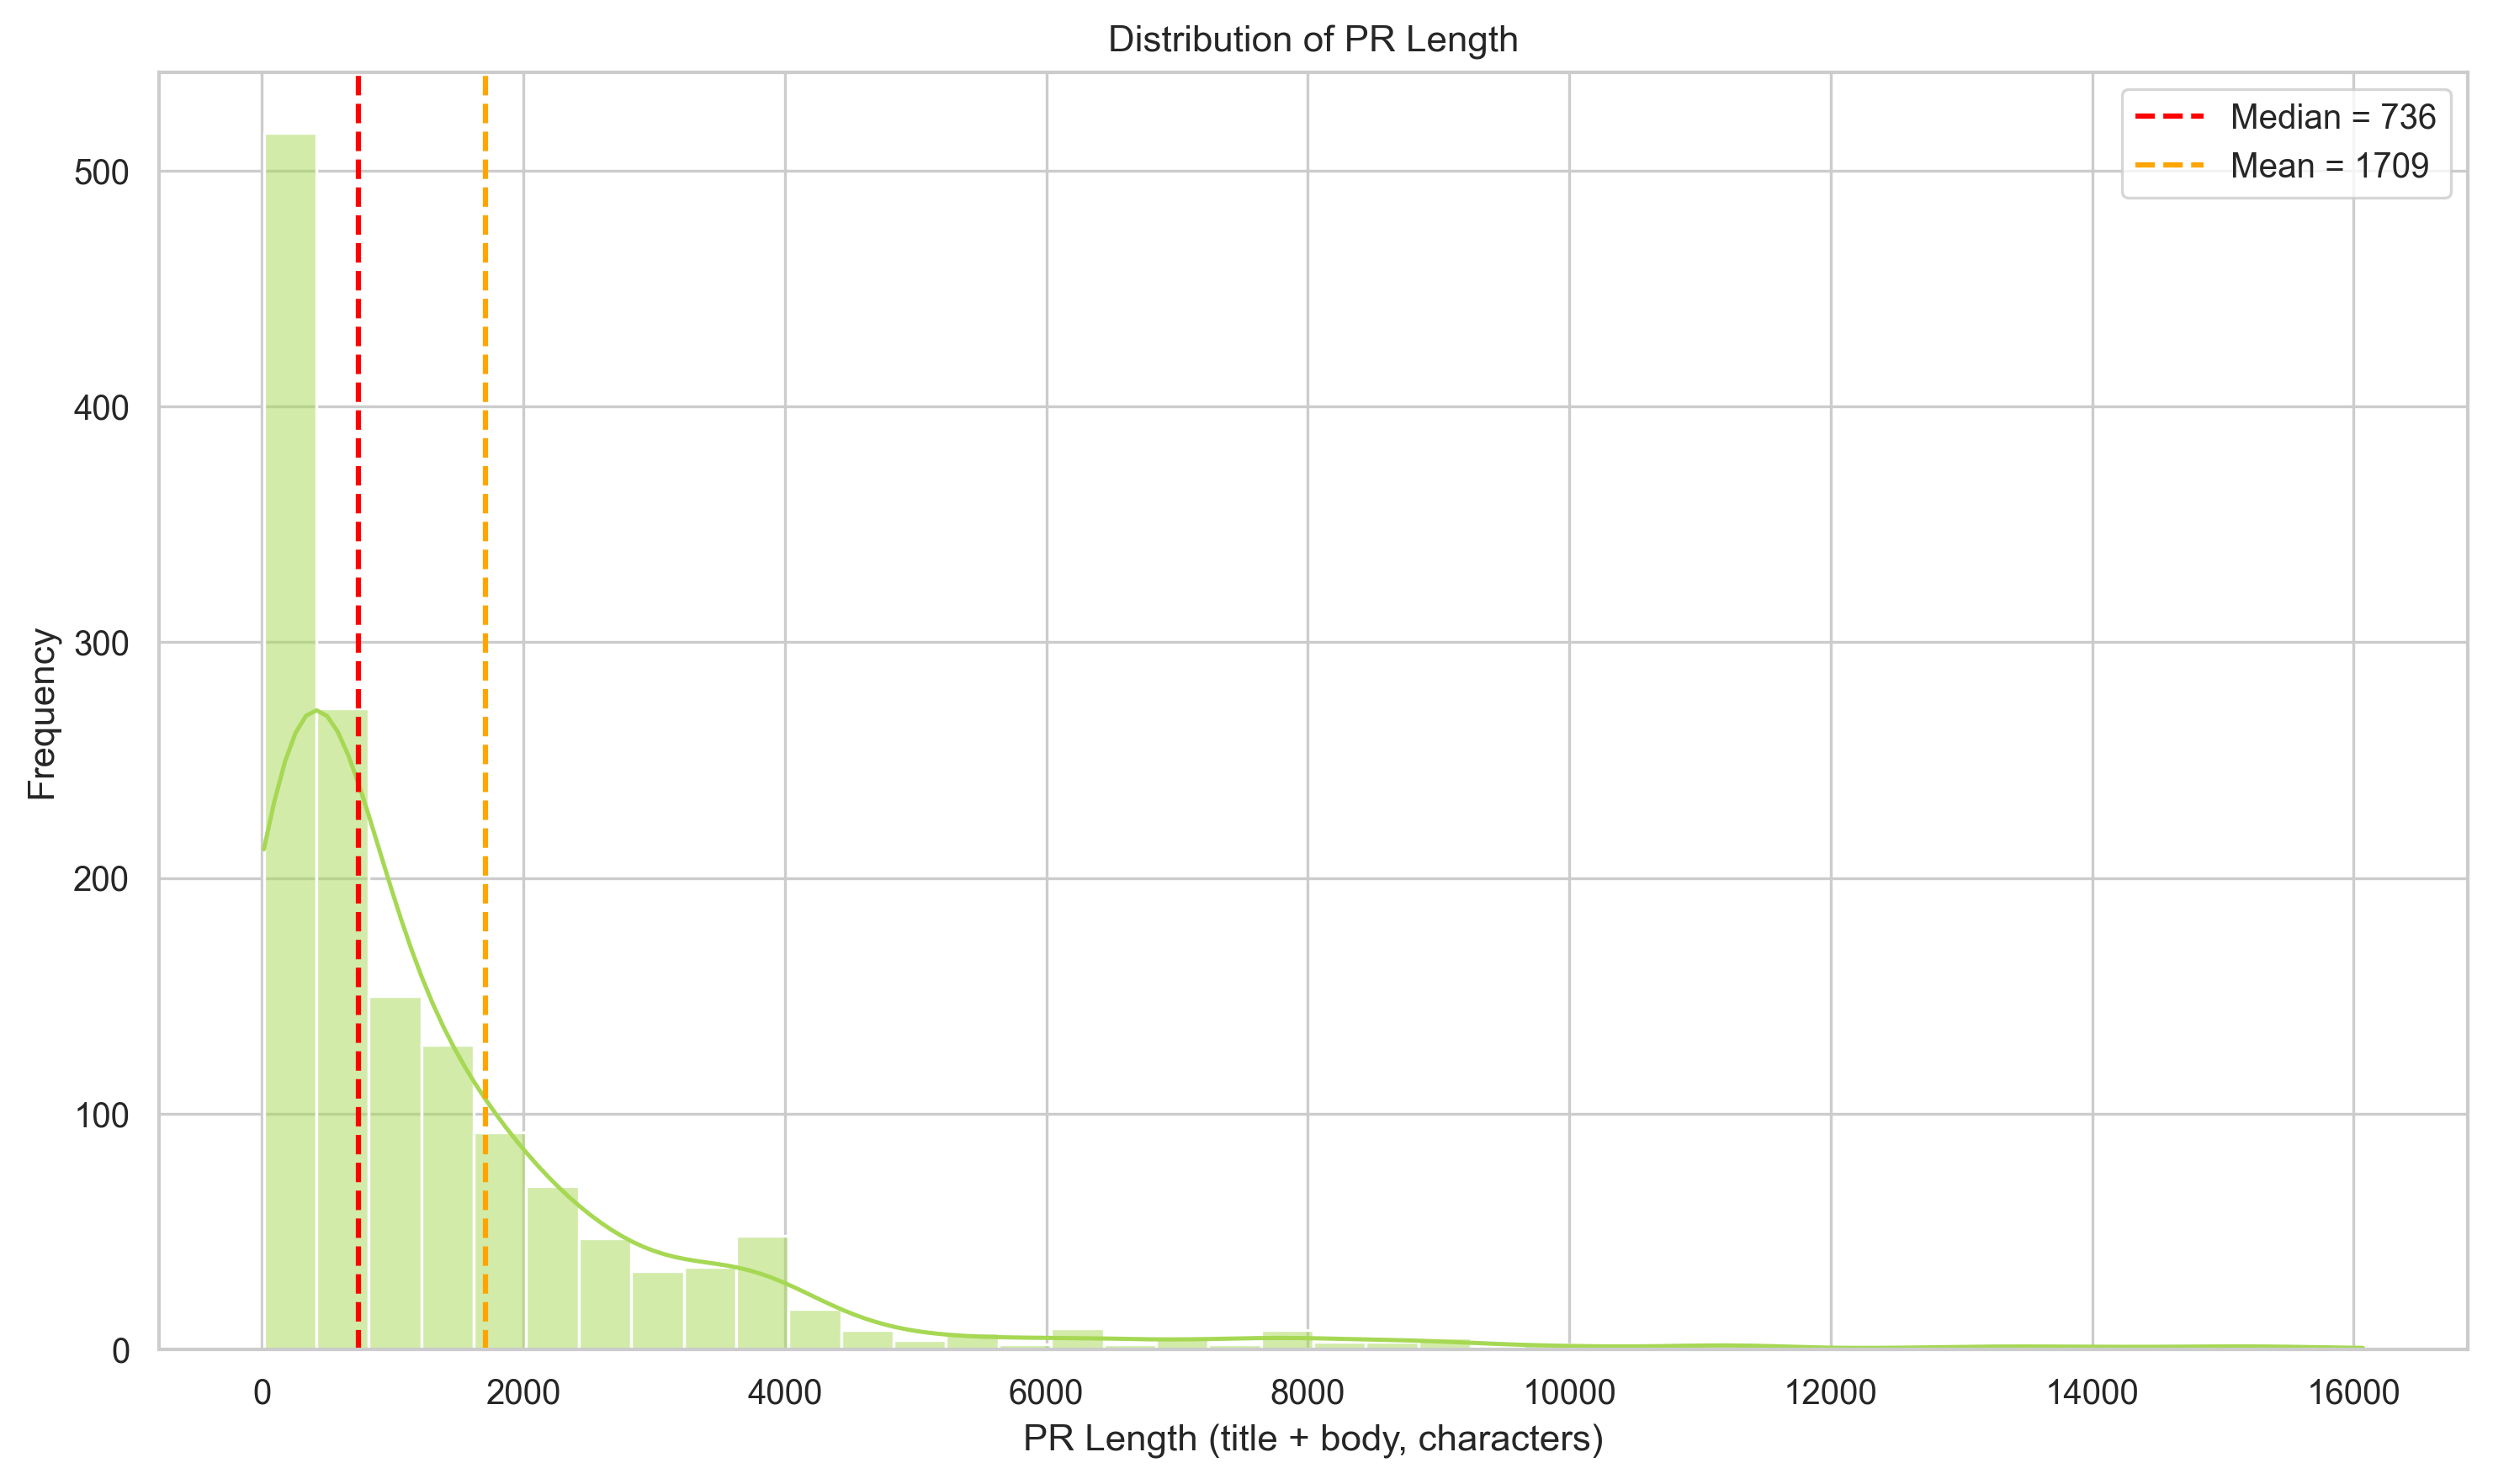
\includegraphics[width=\textwidth]{../figures/05_pr_length_distribution.png}
\caption{PR 长度分布直方图}
\end{figure}

\begin{figure}[ht]
\centering
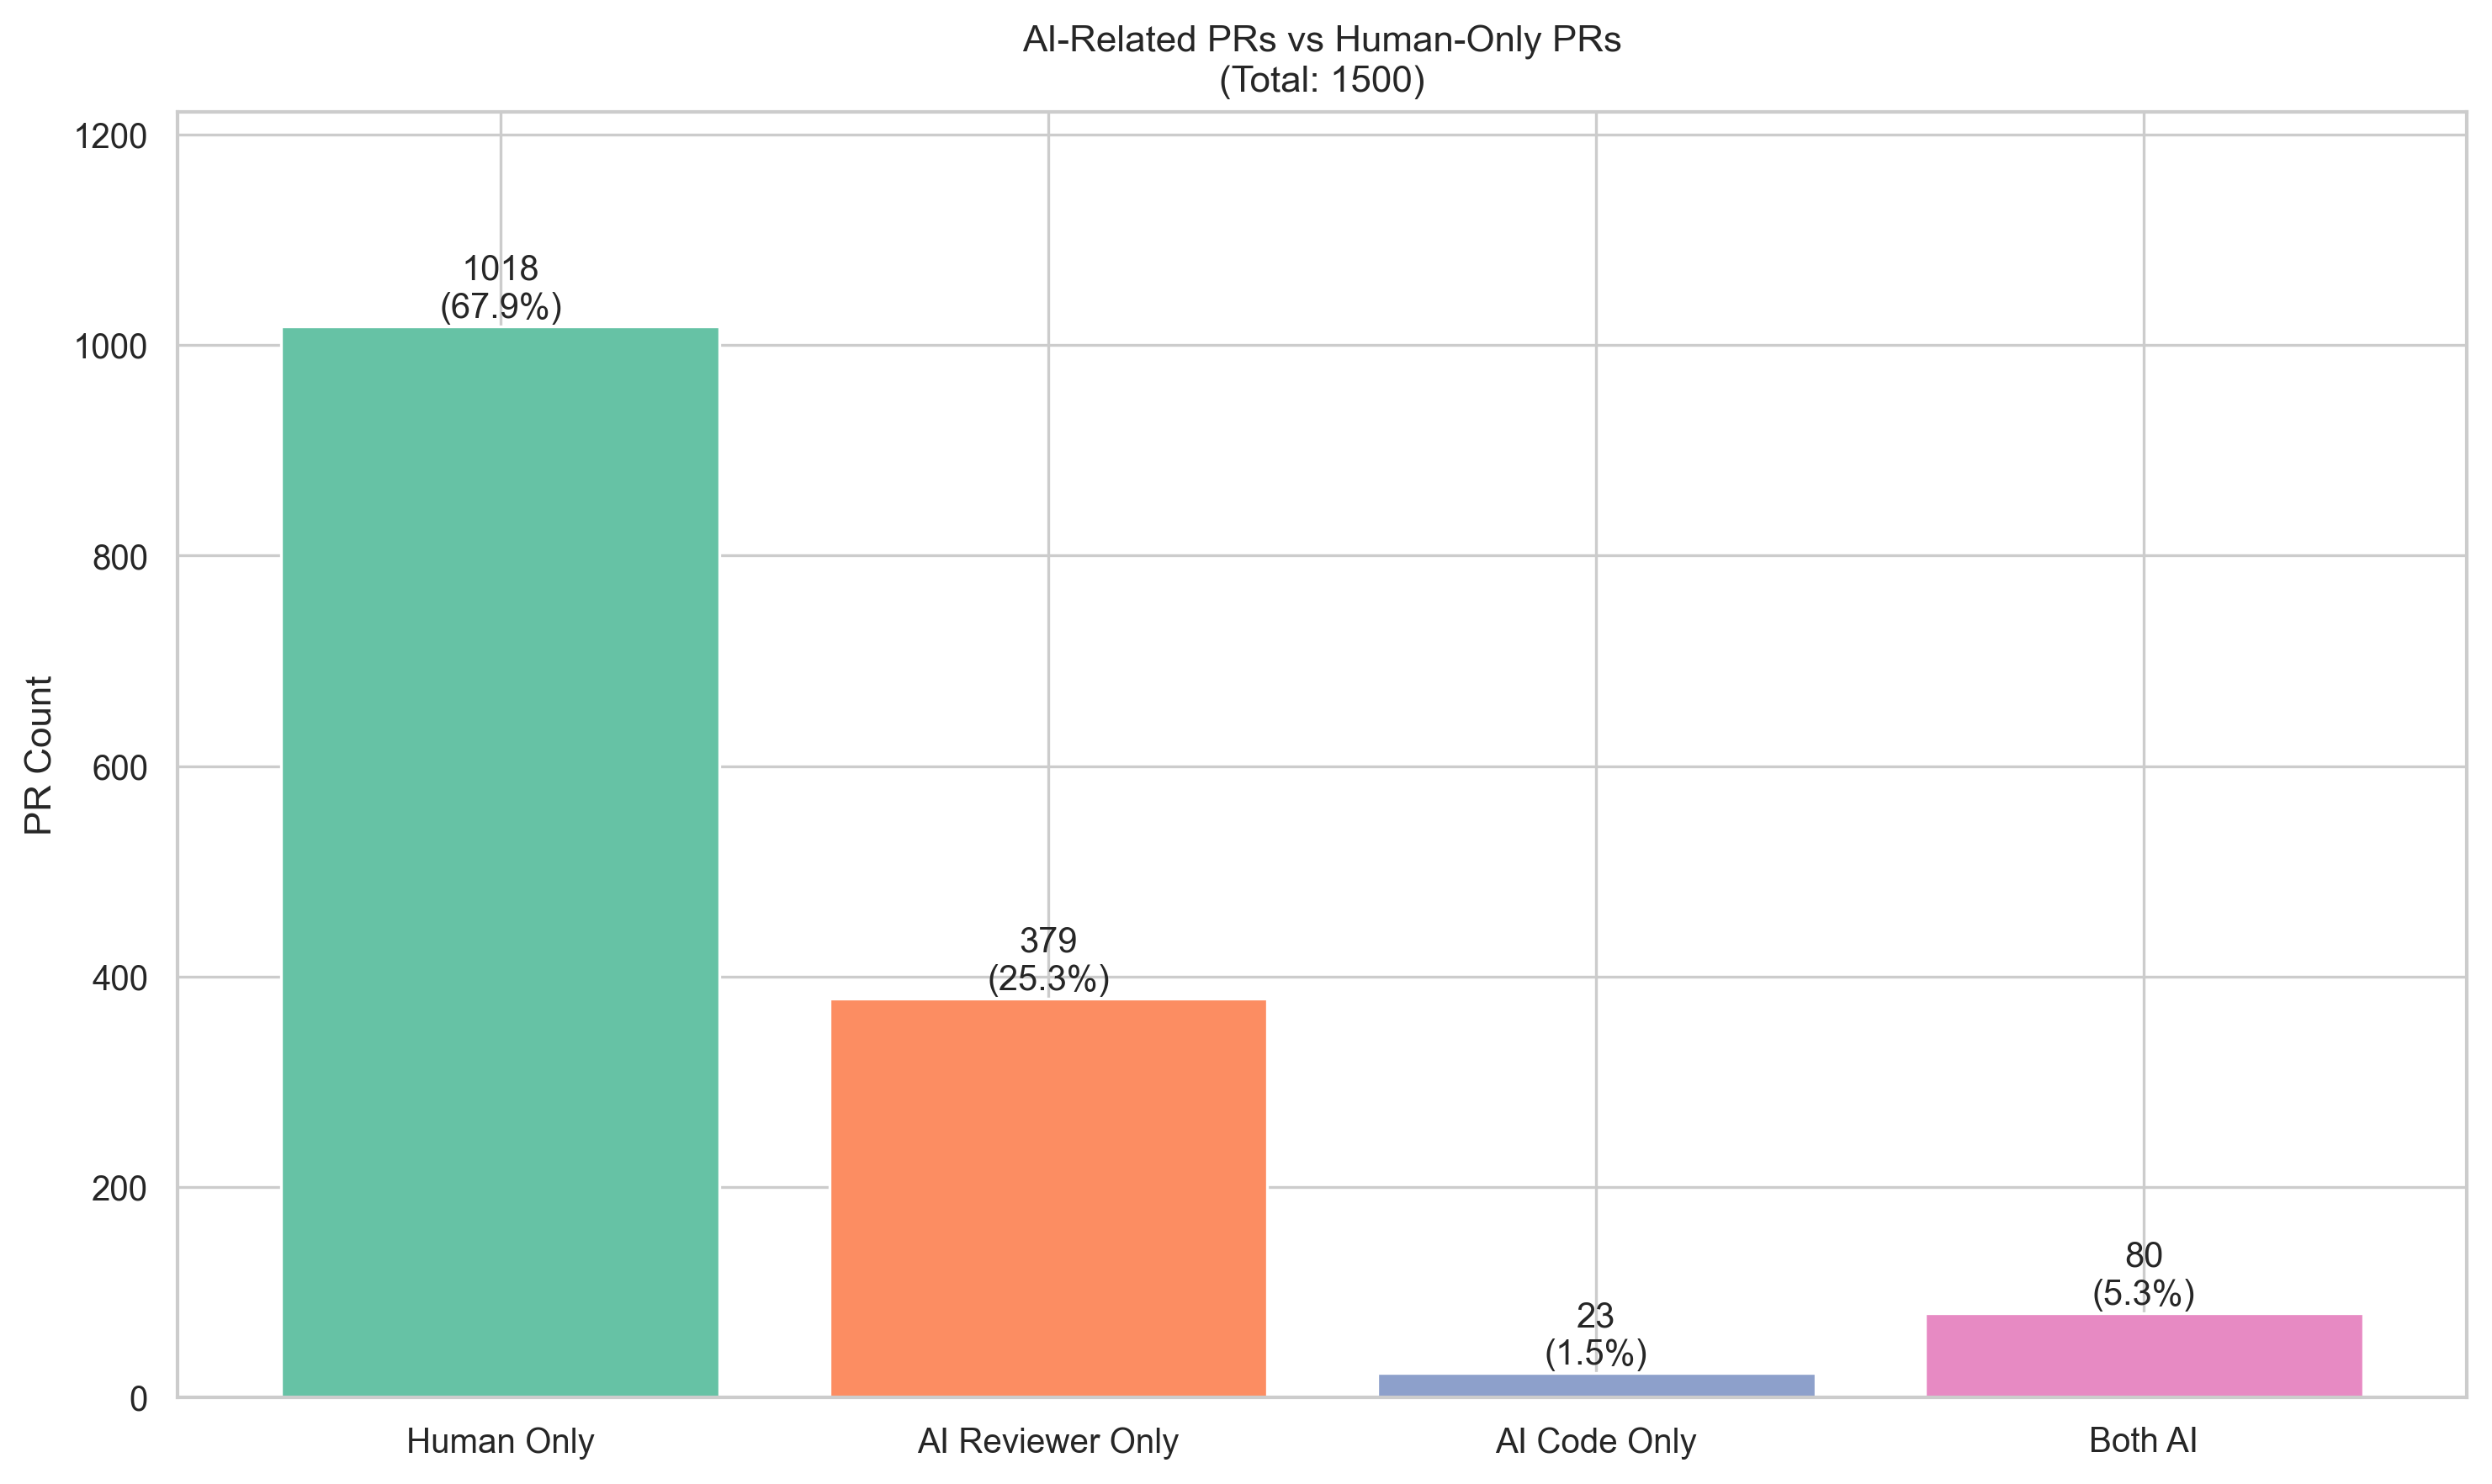
\includegraphics[width=\textwidth]{../figures/06_ai_vs_human_comparison.png}
\caption{AI 相关 PR 与纯人类 PR 数量对比}
\end{figure}

\clearpage
}

%========================
% 实验思考
%========================

\experimentproblems{

\subsection*{4.1 Pull Request 与 Commit 的区别}

Pull Request 是 GitHub 工作流中的一个高层概念，代表一个功能分支向目标分支（如 main）的合并请求。它通常包含多个 Commit，并附有标题、描述、标签、Reviewer 分配、CI 检查结果等元信息。而 Commit 是 Git 版本控制的基本单位，记录一次代码快照的变更。PR 是“请求合并一组 Commits”，而 Commit 是“单次变更的原子记录”。在实际开发中，一个 PR 往往包含多个迭代的 Commit，经过 Review 后可能通过 Squash Merge 合并为单个 Commit。

\subsection*{4.2 Code Review 为何能提高软件质量}

Code Review 通过以下机制提高软件质量：（1）\textbf{知识共享}：团队成员通过审查了解代码变更，减少知识孤岛；（2）\textbf{缺陷发现}：审查者可能发现作者忽略的逻辑错误、边界条件和安全隐患；（3）\textbf{代码规范}：确保代码风格和架构决策符合团队标准；（4）\textbf{可维护性}：促使开发者编写更清晰、更易理解的代码，因为知道会被审查。我们的数据也支持这一点——合并的 PR 修改文件更少、描述更清晰，说明审查过程筛选出了高质量的变更。

\subsection*{4.3 Merge Prediction 的实际应用场景}

Merge Prediction 可应用于：（1）\textbf{CI/CD 资源优化}：优先为高合并概率的 PR 分配 CI 资源；（2）\textbf{开发者辅助}：在 PR 提交前给出改进建议，提高合并成功率；（3）\textbf{项目管理}：预测 PR 的审查周期，帮助团队合理分配 Review 资源；（4）\textbf{开源社区健康度分析}：通过合并率评估项目的审查效率和社区活跃度。

\subsection*{4.4 AI Reviewer 与 Human Reviewer 的差异}

从数据来看，AI Reviewer 占比达 34.9\%，说明 AI 辅助代码审查已相当普遍。可能的差异包括：（1）\textbf{审查速度}：AI 可以秒级完成审查，人类需要数小时到数天；（2）\textbf{关注点}：AI 更多关注语法、风格和安全漏洞，人类更关注业务逻辑和设计决策；（3）\textbf{上下文理解}：AI 对项目全局架构和业务背景的理解有限，人类审查者具备领域知识；（4）\textbf{一致性}：AI 在不同时间给出一致的反馈，人类可能受情绪和疲劳影响。

\subsection*{4.5 数据集类别不平衡问题}

数据集存在一定的类别不平衡（合并率 64.8\%），由各仓库自然合并率差异造成。在后续的 Merge Prediction 任务中，需要注意：（1）\textbf{按仓库分层评估}：VSCode（87.3\%）和 React（48.7\%）的合并率差异可能导致仓库级别的性能差异；（2）\textbf{使用合适的评估指标}：不仅看准确率，还应关注 F1-Score、AUC-ROC 和 PR-AUC；（3）\textbf{可考虑分层采样}：在训练时按仓库和合并状态分层，确保模型学到跨仓库的泛化能力。

\subsection*{4.6 实验中遇到的技术问题}

（1）\textbf{GitHub API 限速}：匿名访问仅 60 次/小时，需要使用 Personal Access Token 将限制提升至 5000 次/小时。（2）\textbf{数据采集速度}：初始串行方案每条约 8 秒，改为 3 线程并行 + PR 内部 5 路并行后，速度提升约 10 倍至 0.8 秒/条。（3）\textbf{采样策略迭代}：初始按更新时间排序导致大量未处理 PR 被选中；改为 closed 状态按创建时间排序后仍存在时间集群效应；最终采用从大池中随机采样的策略，使各仓库合并率更真实。（4）\textbf{TensorFlow 被 Pandas 替换}：发现 TensorFlow 使用 Google 内部审查系统，GitHub 上 99\% 的 PR 无 Review 记录，不适合代码审查研究，替换为审查文化更活跃的 Pandas。（5）\textbf{修改函数提取}：从 Unified Diff 中提取函数名依赖正则表达式，对某些语言（如 C++ 模板）的支持不够完善。
}

%========================
% 实验体会
%========================

\experimentexperience{

通过本次实验，我对 GitHub Pull Request 的数据结构有了系统的认识。从 API 数据采集到特征工程再到统计分析，完整地体验了数据科学项目从 0 到 1 的过程。

主要的收获包括：（1）理解了 PR、Review、Commit 三者之间的层级关系和数据模型；（2）掌握了 GitHub REST API 的分页、限速和认证机制；（3）学会了设计支持断点续传的数据采集流水线，这在处理大规模数据时非常重要；（4）通过特征分析发现了一些有趣的模式——合并的 PR 修改文件更少、描述更简洁，这印证了“小而精”的开源贡献原则。

本次构建的数据集将作为后续实验二至七的基石，为传统机器学习、深度学习和 LLM 方法在代码审查任务上的对比研究提供数据支撑。

}

%========================
% 教师评语
%========================

\teachercomment

\end{document}
